\documentclass{article}
\usepackage[utf8]{inputenc}

% plots
\usepackage{tikz, pgfplots, amsmath}
\usetikzlibrary{positioning,calc,arrows.meta}
\pgfplotsset{compat=1.18} 

% math
\usepackage{amsmath}
\usepackage{amssymb}

\newcommand{\R}{\mathbb{R}}

\begin{document}
Hello

\vspace{1in}


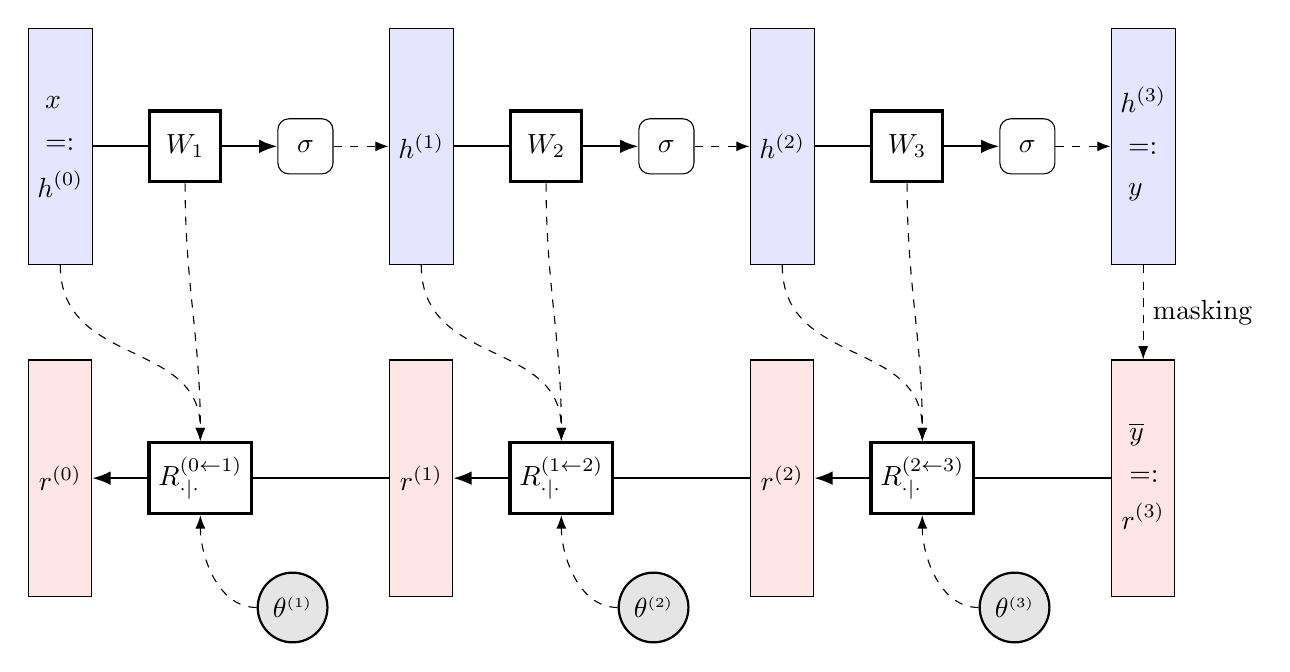
\begin{tikzpicture}[
    vec/.style={rectangle, minimum size=8mm, minimum height=3cm, draw=black, fill=#1},
    vec/.default={blue!10!white},
    mat/.style={rectangle, very thick, draw=black, minimum size=9mm, minimum height=9mm},
    nonl/.style={rectangle, rounded corners, draw=black, minimum size=7mm, minimum height=7mm},
    param/.style={circle, thick, minimum size=20pt, fill=lightgray!40!white, draw=black},
    ]
    \node[vec] (h_0) {
        $\begin{aligned}
            &\;x \\ &=: \\ &h^{(0)}
        \end{aligned}$
    };
    \node[mat, right=0.7cm of h_0] (W1) {$W_1$};
    \node[nonl, right=0.7cm of W1] (nl1) {$\sigma$};
    \node[vec,  right=0.7cm of nl1] (h_1) {$h^{(1)}$};
    \node[mat, right=0.7cm of h_1] (W2) {$W_2$};
    \node[nonl, right=0.7cm of W2] (nl2) {$\sigma$};
    \node[vec,  right=0.7cm of nl2] (h_2) {$h^{(2)}$};
    \node[mat, right=0.7cm of h_2] (W3) {$W_3$};
    \node[nonl, right=0.7cm of W3] (nl3) {$\sigma$};
    \node[vec,  right=0.7cm of nl3] (h_3) {
        $
        \begin{aligned}
            &h^{(3)} \\ &=: \\ &\;y
        \end{aligned}$
    };


    % layer 1 arrows
    \draw[-, thick]                    (h_0.east) to (W1);
    \draw[-{LaTeX[]}, thick]           (W1) to (nl1.west);
    \draw[-{LaTeX[]}, dashed]   (nl1.east) to (h_1.west);
    % layer 2 arrows
    \draw[-, thick]                    (h_1.east) to (W2);
    \draw[-{LaTeX[]}, thick]           (W2) to (nl2.west);
    \draw[-{LaTeX[]}, dashed]   (nl2.east) to (h_2.west);
    % layer 3 arrows
    \draw[-, thick]                    (h_2.east) to (W3);
    \draw[-{LaTeX[]}, thick]           (W3) to (nl3.west);
    \draw[-{LaTeX[]}, dashed]   (nl3.east) to (h_3.west);

    %%% LRP backwards pass %%% 
    %% relevancy vectors
    \node[vec=pink!40!white,  below=1.2cm of h_0] (r_0) {$r^{(0)}$};
    \node[vec=pink!40!white,  below=1.2cm of h_1] (r_1) {$r^{(1)}$};
    \node[vec=pink!40!white,  below=1.2cm of h_2] (r_2) {$r^{(2)}$};
    \node[vec=pink!40!white,  below=1.2cm of h_3] (r_3) {
        $\begin{aligned}
            & \;\overline{y}\\ &=: \\ &r^{(3)}
        \end{aligned}$
    };

    %% arrow to output layer relevancies
    \draw[-{LaTeX[]}, dashed]   (h_3.south) to node[right] {masking} (r_3.north);

    %% conditional relevancy matrices
    \node[mat, right=0.7cm of r_0] (R1) {$R^{(0 \leftarrow 1)}_{\cdot | \cdot}$};
    \node[mat, right=0.7cm of r_1] (R2) {$R^{(1 \leftarrow 2)}_{\cdot | \cdot}$};
    \node[mat, right=0.7cm of r_2] (R3) {$R^{(2 \leftarrow 3)}_{\cdot | \cdot}$};
    
    %% arrows towards conditional relevancy matrices
    % layer 1 arrows
    \draw[-{LaTeX[]}, dashed]   (h_0.south) .. controls +(down:13mm) and +(up:13mm) .. (R1.north);
    \draw[-{LaTeX[]}, dashed]   (W1.south)  .. controls +(down:13mm) and +(up:13mm) .. (R1.north);
    % layer 2 arrows
    \draw[-{LaTeX[]}, dashed]   (h_1.south) .. controls +(down:13mm) and +(up:13mm) .. (R2.north);
    \draw[-{LaTeX[]}, dashed]   (W2.south)  .. controls +(down:13mm) and +(up:13mm) .. (R2.north);
    % layer 3 arrows
    \draw[-{LaTeX[]}, dashed]   (h_2.south) .. controls +(down:13mm) and +(up:13mm) .. (R3.north);
    \draw[-{LaTeX[]}, dashed]   (W3.south)  .. controls +(down:13mm) and +(up:13mm) .. (R3.north);
    
    %% arrows of LRP backward pass
    % layer 1 arrows
    \draw[-, thick]            (r_1.west) to (R1);
    \draw[-{LaTeX[]}, thick]   (R1) to (r_0.east);
    % layer 2 arrows
    \draw[-, thick]            (r_2.west) to (R2);
    \draw[-{LaTeX[]}, thick]   (R2) to (r_1.east);
    % layer 3 arrows
    \draw[-, thick]            (r_3.west) to (R3);
    \draw[-{LaTeX[]}, thick]   (R3) to (r_2.east);

    %% params
    \node[param, below right=12mm of R1.south] (param1) {$\theta^\text{\tiny{{(1)}}}$};
    \node[param, below right=12mm of R2.south] (param2) {$\theta^\text{\tiny{{(2)}}}$};
    \node[param, below right=12mm of R3.south] (param3) {$\theta^\text{\tiny{{(3)}}}$};

    %% arrows towards conditional relevancy matrices
    \draw[-{LaTeX[]}, dashed]   (param1.west) .. controls +(left:5mm) and +(down:5mm) .. (R1.south);
    \draw[-{LaTeX[]}, dashed]   (param2.west) .. controls +(left:5mm) and +(down:5mm) .. (R2.south);
    \draw[-{LaTeX[]}, dashed]   (param3.west) .. controls +(left:5mm) and +(down:5mm) .. (R3.south);

\end{tikzpicture}

\vspace{1in}

% \resizebox{\textwidth}{!}{%
\begin{figure}
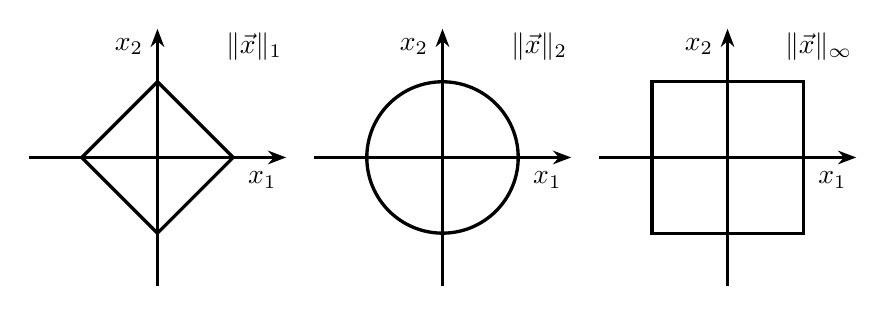
\begin{tikzpicture}[]
    \begin{axis}
        [
            name=a,
            height=0.4\textwidth, width=0.4\textwidth,
            xmin=-1.7, xmax=1.7, ymin=-1.7, ymax=1.7, 
            axis lines=middle, axis line style={thick, -{Stealth[scale=1]}},
            xtick={0}, ytick={0},
            xlabel=$x_1$, xlabel style={below=(.06cm of current axis.right of origin), anchor=north east},
            ylabel=$x_2$, ylabel style={left=(.06cm of current axis.above origin), anchor=north east},
        ]
        \draw[style=very thick] ( 1,0) -- (0,-1);
        \draw[style=very thick] (-1,0) -- (0,-1);
        \draw[style=very thick] ( 1,0) -- (0, 1);
        \draw[style=very thick] (-1,0) -- (0, 1);

        % label
        \node[below left=-.1cm of current axis.north east] {$\| \vec{x} \|_1$};
    \end{axis}
    \begin{axis}
        [
            name=b, at=(a.south east), xshift=1em, 
            height=0.4\textwidth, width=0.4\textwidth,
            xmin=-1.7, xmax=1.7, ymin=-1.7, ymax=1.7, 
            axis lines=middle, axis line style={thick, -{Stealth[scale=1]}},
            xtick={0}, ytick={0},
            xlabel=$x_1$, xlabel style={below=(.06cm of current axis.right of origin), anchor=north east},
            ylabel=$x_2$, ylabel style={left=(.06cm of current axis.above origin), anchor=north east},
        ]
        \draw[style=very thick] (0,0) circle (1);

        % label
        \node[below left=-.1cm of current axis.north east] {$\| \vec{x} \|_2$};
    \end{axis}
    \begin{axis}
        [
            name=c, at=(b.south east), xshift=1em, 
            height=0.4\textwidth, width=0.4\textwidth,
            xmin=-1.7, xmax=1.7, ymin=-1.7, ymax=1.7, 
            axis lines=middle, axis line style={thick, -{Stealth[scale=1]}},
            xtick={0}, ytick={0},
            xlabel=$x_1$, xlabel style={below=(.06cm of current axis.right of origin), anchor=north east},
            ylabel=$x_2$, ylabel style={left=(.06cm of current axis.above origin), anchor=north east},
        ]
        \draw[style=very thick] (-1,-1) rectangle (1,1);
        
        % label
        \node[below left=-.1cm of current axis.north east] {$\| \vec{x} \|_\infty$};
    \end{axis}
\end{tikzpicture}
\caption[]{Unit circles of three vector norms on $\R^2$};
\end{figure}
% }

\end{document}
